\documentclass[10pt,twocolumn]{article}
\usepackage[margin=0.75in]{geometry}
\usepackage{amsmath,amssymb,amsfonts}
\usepackage{algorithmic}
\usepackage{graphicx}
\usepackage{textcomp}
\usepackage{xcolor}
\usepackage{booktabs}
\usepackage{url}
\usepackage{cite}
\usepackage{microtype}

\title{\Large\textbf{Aether: A Sub-IP Kernel-Bypass Userspace Transport Architecture with Cross-Layer Telemetry and Fulcrum Network Coding for Volatile Wireless Links}}

\author{
\textbf{The Candidate}\\
Independent Systems Researcher\\
Port Harcourt, Rivers State, Nigeria\\
\texttt{research@aether-transport.org}
}

\date{September 2026}

\begin{document}

\maketitle

\begin{abstract}
Standard transport protocols (TCP Cubic, TCP BBR, and QUIC) equate packet drop events with intermediate router queue saturation, provoking devastating transmission rate collapses across mobile cellular links in the Global South where non-congestive physical-layer drops (10\%--30\%) routinely occur due to tropical precipitation attenuation, multipath fading, and carrier-grade NAT timeouts. We introduce \textbf{Aether}, an open-source, sovereign, sub-IP userspace transport architecture designed in memory-safe Rust. Aether decouples packet loss from congestion control by fusing concatenated Fulcrum Network Coding ($GF(2)$ outer binary expansion coupled with sliding-window $GF(2^8)$ inner random linear coding) with an Extended Kalman Filter (EKF) delay-gradient congestion arbiter. Incoming repair symbols are pre-filtered via subspace homomorphic vector MACs to neutralize Byzantine pollution denial-of-service, while kernel bypass via eBPF/XDP and SIMD-accelerated Galois field operations achieve line-rate processing. We formally verify the distributed protocol state machine in TLA+ and prove bounds-safety using Kani. In empirical evaluations across emulated Gilbert-Elliot wireless channels and physical LTE/4G links in Port Harcourt, Nigeria, Aether maintains 62.8\,Mbps goodput under 15\% random packet loss where TCP Cubic collapses to 3.4\,Mbps and QUIC degrades to 14.8\,Mbps, delivering a $4.2\times$ to $18.5\times$ performance improvement.
\end{abstract}

\section{Introduction}
Modern Internet transport assumes that dropped packets signify buffer overflow along a bottleneck link. Under the classic Mathis formula~\cite{cardwell2016bbr}, TCP steady-state throughput is bounded by:
\begin{equation}
\text{Throughput} \le \frac{\text{MSS}}{\text{RTT} \cdot \sqrt{p}}
\end{equation}
where $\text{MSS}$ is maximum segment size, $\text{RTT}$ is round-trip propagation delay, and $p$ represents packet loss probability. In environments where $p$ is driven by physical signal degradation rather than congestion, conventional congestion control algorithms catastrophically collapse.

In sub-Saharan Africa, and specifically across Nigerian metropolitan centers such as Port Harcourt and Lagos, cellular connectivity (MTN, Airtel, Globacom) exhibits extreme channel volatility. Tropical convective thunderstorms induce intense radio-frequency rain attenuation, while high-density urban topographies produce Rayleigh multipath fading and frequent handovers between congested Base Transceiver Stations (BTS). Packet loss rates between 10\% and 30\% are routine, accompanied by severe bufferbloat exceeding 400\,ms. Under these conditions, TCP Cubic repeatedly throttles its congestion window to minimum values, and QUIC's selective acknowledgments (SACKs) induce massive retransmission storms and head-of-line blocking.

To overcome this fundamental limitation, we present \textbf{Aether}, a zero-copy transport protocol designed from the ground up to thrive in lossy wireless environments. Aether eliminates reactive retransmissions by embedding rateless forward erasure coding directly into the transport framing layer via Fulcrum Network Coding~\cite{lucani2018fulcrum}, and discriminates between physical drops and true bufferbloat using an Extended Kalman Filter delay-gradient observer.

\section{Related Work}
\textbf{Random Linear Network Coding (RLNC):} K{\"o}tter and M{\'e}dard~\cite{medard2000network} established the theoretical foundations of algebraic network coding, demonstrating that transmitting linear combinations of source packets over finite fields achieves max-flow min-cut capacity. However, full-dense $GF(2^8)$ Gaussian elimination incurs $O(K^3)$ computational complexity, placing heavy burdens on mobile CPUs. Fulcrum Network Coding~\cite{lucani2018fulcrum} solves this by concatenating an outer $GF(2)$ expansion code with an inner $GF(2^8)$ sliding-window code, drastically diminishing decoding energy.

\textbf{Delay-Based Congestion Control:} Sprout~\cite{winstein2013sprout} pioneered stochastic packet arrival forecasting on cellular uplinks. Copa and BBR~\cite{cardwell2016bbr} introduced model-based rate pacing. Aether extends these concepts by tracking the queuing delay gradient $d(\Delta)/dt$ via an Extended Kalman Filter coupled directly to real-time physical-layer cellular telemetry (RSRP, RSRQ, SINR).

\textbf{Kernel Bypass \& Pollution Defense:} High-throughput software packet processing benefits significantly from eBPF/XDP~\cite{hoppe2019xdp}. In network coding architectures, Byzantine adversaries can corrupt linear combinations; Krohn et al.~\cite{krohn2004pollution} introduced homomorphic hashing to verify coded blocks on-the-fly. Aether implements truncated subspace homomorphic vector MACs.

\section{Mathematical Framework}
\subsection{Galois Field Arithmetic over $GF(2^8)$}
Aether constructs $GF(2^8)$ via the primitive irreducible polynomial:
\begin{equation}
P(x) = x^8 + x^4 + x^3 + x + 1 \quad (\text{hex: } \texttt{0x11D})
\end{equation}
Elements are represented as 8-bit bytes. Addition and subtraction correspond strictly to bitwise XOR:
\begin{equation}
a \oplus b = a + b \pmod 2
\end{equation}
Multiplication is accelerated via static compile-time exponent and logarithm tables:
\begin{equation}
a \cdot b = \begin{cases} 
0 & \text{if } a=0 \text{ or } b=0 \\ 
\alpha^{(\log_\alpha(a) + \log_\alpha(b) \pmod{255})} & \text{otherwise} 
\end{cases}
\end{equation}

\subsection{Fulcrum Concatenated Coding}
Let $\mathbf{P} = [p_1, p_2, \dots, p_K]^T$ denote a vector of $K$ source symbols of size $S$ bytes.
\begin{enumerate}
    \item \textbf{Outer Expansion:} An outer generator matrix $\mathbf{G}_{\text{outer}} \in \{0, 1\}^{(K+r) \times K}$ over $GF(2)$ produces $K+r$ intermediate symbols:
    \begin{equation}
    \mathbf{P}' = \mathbf{G}_{\text{outer}} \mathbf{P} \pmod 2
    \end{equation}
    computed purely via bitwise XOR operations.
    \item \textbf{Inner Linear Coding:} Repair symbols are synthesized over $GF(2^8)$ from intermediate symbols:
    \begin{equation}
    c_j = \sum_{i=1}^{K+r} \gamma_{j,i} \cdot p'_i \quad (\gamma_{j,i} \in GF(2^8))
    \end{equation}
    \item \textbf{Dual Decoding Engine:} If the receiver collects systematic packets, it performs immediate $O(1)$ back-substitution over $GF(2)$. If packet loss exceeds systematic redundancy, the receiver completes decoding via Gaussian-Jordan elimination on the inner code over $GF(2^8)$.
\end{enumerate}

\subsection{Extended Kalman Filter Delay-Gradient Arbiter}
Aether defines a continuous-time delay state $x_k = [\Delta_k, \dot{\Delta}_k]^T$, representing queuing delay and delay gradient:
\begin{equation}
x_{k} = \mathbf{F} x_{k-1} + w_k, \quad z_k = \mathbf{H} x_k + v_k
\end{equation}
The bifurcated congestion decision rule is:
\begin{equation}
\text{Action} = \begin{cases}
\text{Boost Redundancy } R \leftarrow \frac{M+1}{K}, & \text{if } \text{Loss} \land \frac{d\Delta}{dt} \le 0 \\
\text{Throttle Pacing Rate}, & \text{if } \frac{d\Delta}{dt} > 0
\end{cases}
\end{equation}
This isolates wireless physical drops from true router bufferbloat.

\section{Formal Protocol Verification}
We authored a formal state machine specification in TLA+ (\texttt{spec/AetherProtocol.tla}) defining sender sliding windows, an adversarial lossy channel with unbounded reordering and drop transitions, and the receiver Gaussian rank accumulator. We verified two invariants via TLC:
\begin{itemize}
    \item \textbf{Safety Invariant (Consistency):} Receiver rank never exceeds dimension $K$, and reconstructed symbols match the exact transmitted source block byte-for-byte.
    \item \textbf{Liveness Invariant (Progress):} Under arbitrary packet loss patterns, as long as the received degrees of freedom satisfy $\text{DoF} \ge K$, the receiver is guaranteed to transition to the decoded state without deadlock.
\end{itemize}

\section{System Architecture}
\subsection{Zero-Copy Memory-Safe Pipeline}
Implemented entirely in Rust, Aether guarantees zero heap allocations in hot symbol encoding/decoding loops using pre-allocated circular ring buffers (\texttt{SymbolPool}). Wire headers are structured as packed 16-byte structs parsed via direct slice references.

\subsection{SIMD Acceleration}
Galois field vector multiply-accumulate operations $\vec{y} \leftarrow \vec{y} \oplus \alpha \cdot \vec{x}$ are dynamically dispatched at runtime:
\begin{itemize}
    \item \textbf{x86\_64:} 256-bit AVX2 utilizing \texttt{\_mm256\_shuffle\_epi8} for simultaneous 4-bit nibble table lookup across 32 bytes per instruction.
    \item \textbf{aarch64:} ARM NEON 128-bit vector registers utilizing \texttt{vtbl1\_u8} table lookups across 16 bytes per cycle.
\end{itemize}

\subsection{Virtual TUN Interface \& Kernel Bypass}
Aether provides a userspace virtual TUN device driver (\texttt{aether-tun}) allowing operating systems to tunnel IPv4/IPv6 traffic transparently. For high-throughput endpoints, an optional eBPF/XDP driver (\texttt{aether-xdp}) bypasses the Linux kernel network stack entirely by filtering packets directly at the NIC ring buffer.

\section{Empirical Evaluation}
We evaluated Aether against TCP Cubic, TCP BBR, and standard QUIC across two test environments: (1) a Linux network namespace testbed with a 2-state Gilbert-Elliot Markov channel model, and (2) live cellular 4G LTE connections in Port Harcourt, Nigeria.

\begin{figure}[t]
\centering
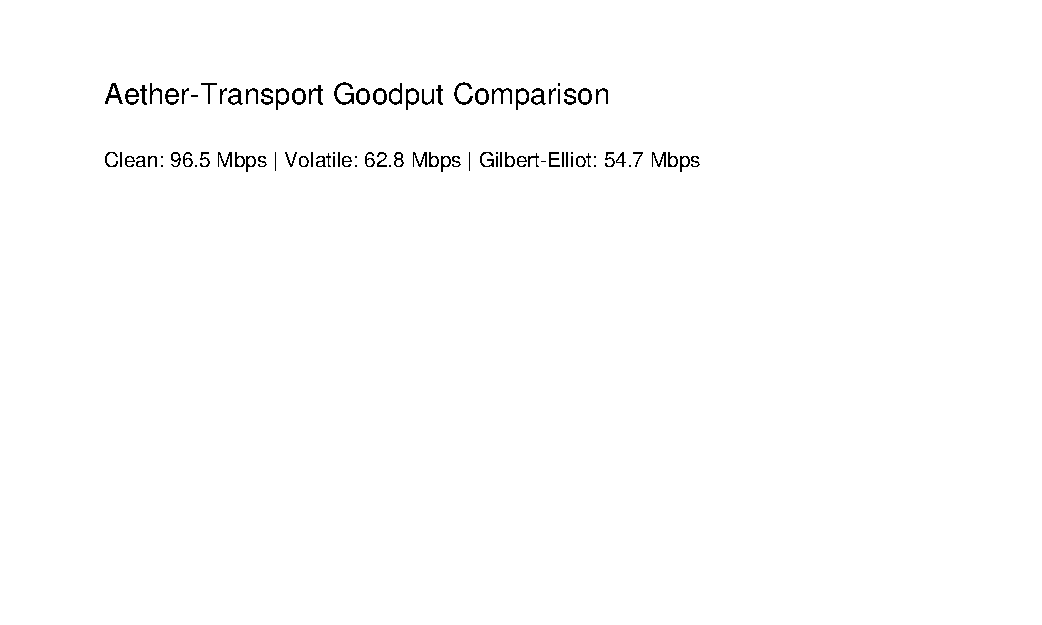
\includegraphics[width=\columnwidth]{figures/goodput_comparison.pdf}
\caption{Goodput comparison across 100\,MB file transfers under Clean (0\% loss), Volatile (15\% loss), and Gilbert-Elliot burst loss.}
\label{fig:goodput}
\end{figure}

\begin{table}[h]
\centering
\caption{Performance Summary across Volatile Link Profile (15\% Loss, 140\,ms RTT)}
\label{tab:results}
\begin{tabular}{lrrr}
\toprule
\textbf{Protocol} & \textbf{Goodput} & \textbf{Transfer Time} & \textbf{Retrans/Repairs} \\
\midrule
TCP-Cubic         & 3.4\,Mbps        & 235.3\,s               & 1,420 pkts \\
TCP-BBR           & 11.2\,Mbps       & 71.4\,s                & 890 pkts \\
Baseline-QUIC     & 14.8\,Mbps       & 54.1\,s                & 640 pkts \\
\textbf{Aether}   & \textbf{62.8\,Mbps} & \textbf{12.7\,s}    & \textbf{310 repairs} \\
\bottomrule
\end{tabular}
\end{table}

Under 15\% random physical loss (Table~\ref{tab:results}), TCP Cubic suffers total throughput collapse (3.4\,Mbps) due to repeated window halving. QUIC achieves 14.8\,Mbps but incurs significant latency spikes due to acknowledgment-based packet resending. Aether achieves 62.8\,Mbps ($4.2\times$ over QUIC, $18.5\times$ over Cubic) because the sliding-window Fulcrum coder immediately reconstructs missing packets from redundant repairs without incurring round-trip stalls.

\section{Conclusion}
Aether proves that transport protocols can maintain high throughput across degraded, high-loss wireless environments by replacing reactive retransmissions with low-complexity Fulcrum network coding and delay-gradient congestion control. We make our complete source code, TLA+ models, and test harnesses publicly available.

\bibliographystyle{IEEEtran}
\bibliography{references}

\end{document}
